\documentclass[10pt]{scrartcl}

\usepackage[utf8]{inputenc}
\usepackage{tabularx}
\usepackage{longtable}
\usepackage[ngerman]{babel}
\usepackage[automark]{scrpage2}
\usepackage{amsmath,amssymb,amstext}
%\usepackage{mathtools}
\usepackage[]{color}
\usepackage[]{enumerate}
\usepackage{graphicx}
\usepackage{lastpage}
\usepackage[perpage,para,symbol*]{footmisc}
\usepackage{listings} 
\usepackage[pdfborder={0 0 0},colorlinks=false]{hyperref}
\usepackage[numbers,square]{natbib}
\usepackage{color}
\usepackage{colortbl}
\usepackage[absolute]{textpos}
\usepackage{float}
\usepackage[colorinlistoftodos,textsize=small,textwidth=2cm,shadow,bordercolor=black,backgroundcolor={red!100!green!33},linecolor=black]{todonotes}

\lstset{numbers=left, numberstyle=\tiny, numbersep=5pt, breaklines=true, showstringspaces=false} 
\restylefloat{figure}

%changehere
\def\titletext{Praktikum 4 : Experimente}
\def\titletextshort{Praktikum 4}
\author{André Harms, Oliver Steenbuck, Armin Steudte  \\ Carsten Noetzel, Dennis Blauhut, Torben Becker}

\title{\titletext}

%changehere Datum der Übung
\date{11.01.2012}

\pagestyle{scrheadings}
%changehere
\ihead{MI, Thiel-Clemen}
\ifoot{Generiert am:\\ \today}

\cfoot{Oliver Steenbuck, André Harms \\  Armin Steudte, Carsten Noetzel \\ Dennis Blauhut, Torben Becker}


\ohead[]{\titletextshort}
\ofoot[]{{\thepage} / \pageref{LastPage}}

\setlength{\parindent}{0.0in}
\setlength{\parskip}{0.1in}

\begin{document}
\maketitle

\setcounter{tocdepth}{3}
\tableofcontents

	\listoftables                                 												% 
	\listoffigures   

\section{Anleitung zur Simulation}

\subsection{Ausführung}
Die beiliegende sim.tar.gz entpacken und den Anweisungen in der readme.txt folgen.
In dieser wird beschrieben wie die jvm mit den nativen lwjgl (Linux Lightweight Game Library) Bibliotheken gestartet werden kann. Die Simulation läuft dann von alleine ab.
\subsection{Export}
Ergebniss der Simulation ist eine csv Datei \verb!gamelog.csv! die im Ordner liegt von dem aus die Simulation gestartet wurde.


\subsection{Sourcen}
Das Project ist in Eclipse entwickelt als build tool kommt Maven zum Einsatz. Die sourcen incl. Eclipse Projektkonfigurationen sind auf githup (\verb!https://github.com/MyersGer/WS_2011/tree/master/MIP/Praktikum%202/MI_SIM_MAVEN!).

\subsubsection{Maven Konfiguration}
Da slick leider nicht für Maven verfügbar ist müßen die betreffenden Bibliotheken manuell in die systemlokalen repositories geladen werden. Die betreffenden Kommandos sind in der Datei \verb!dependecyAdder.txt! im Projectroot enthalten.

\subsubsection{Native libs}
Auch für das ausführen aus eclipse müßen die nativen lwjgl Bibliotheken eingebunden werden. In der Version im repository sind die linux libs eingebunden. Alle nativen libraries befinden sich im project in \verb!src/main/resources/lwjgl/native!. Es exisitert hier jeweils ein Ordner pro unterstütztem OS.

Um die native libraries einzubinden gibt es zwei Wege, einmal über die GUI und einmal direkt im config file. Wir empfehlen das config file.

\subsubsection{GUI}
Die betreffendne Konfiguration findet sich in eclipse im Kontextmenü des Projektes. BuildPath $\rightarrow$ configure buildpath $\rightarrow$ fenster öffnet sich $\rightarrow$ linksJava Build Path auswählen $\rightarrow$ Tab Libraries $\rightarrow$ aufklappen lwjgl.jar $\rightarrow$ Native library location $\rightarrow$ edit

\subsubsection{Config File}
Im projectroot öffnen der Datei \verb!.classpath! anpassen von:\begin{verbatim}


	<classpathentry kind="lib" path="src/main/resources/lib/lwjgl.jar">
		<attributes>
			<attribute name="org.eclipse.jdt.launching.CLASSPATH_ATTR_LIBRARY_PATH_ENTRY" 
			value="MI_SIM_MAVEN/src/main/resources/lwjgl/native/linux"/>
		</attributes>
	</classpathentry> 
\end{verbatim}

Es müßte hier zum wechsel auf einen Mac \verb!linux! durch \verb!macosx! ersetzt werden.

\section{Versuchsdurchführung}
Die Versuchsdurchführung erfolgte gemäß der Fragestellung. Zunächst wurde der IST-Zustand des Campus modelliert und die Simulation durchgeführt um die Ausgangswerte zur Bewertung des Ergebnisse zu erhalten. Im Anschluss wurden Maßnahmen zur Verbesserung bzw. Verschlechterung des Campus getroffen und die Simulationsergebnisse mit dem IST-Zustand verglichen.\\
Betrachtet wird der Weg von der U-Bahn Lohmühlenstrasse durch das blaue Haus hin zu IT-Hochhaus (in den Grafiken ist dies durch den roten Weg zu erkennen).

\subsection{IST-Zustand des Campus}
Abbildung \ref{img:IST} zeigt den IST-Zustand des Campus. Hierbei ist der Abwasserkanal rund um das blaue Haus zu beachten und der schmale, schlecht beleuchtete Gang im blauen Haus, welche beide Einfluss auf die Simulationsergebnisse haben (siehe \ref{sec:Ergebnisse}).

	\begin{figure}[H]
                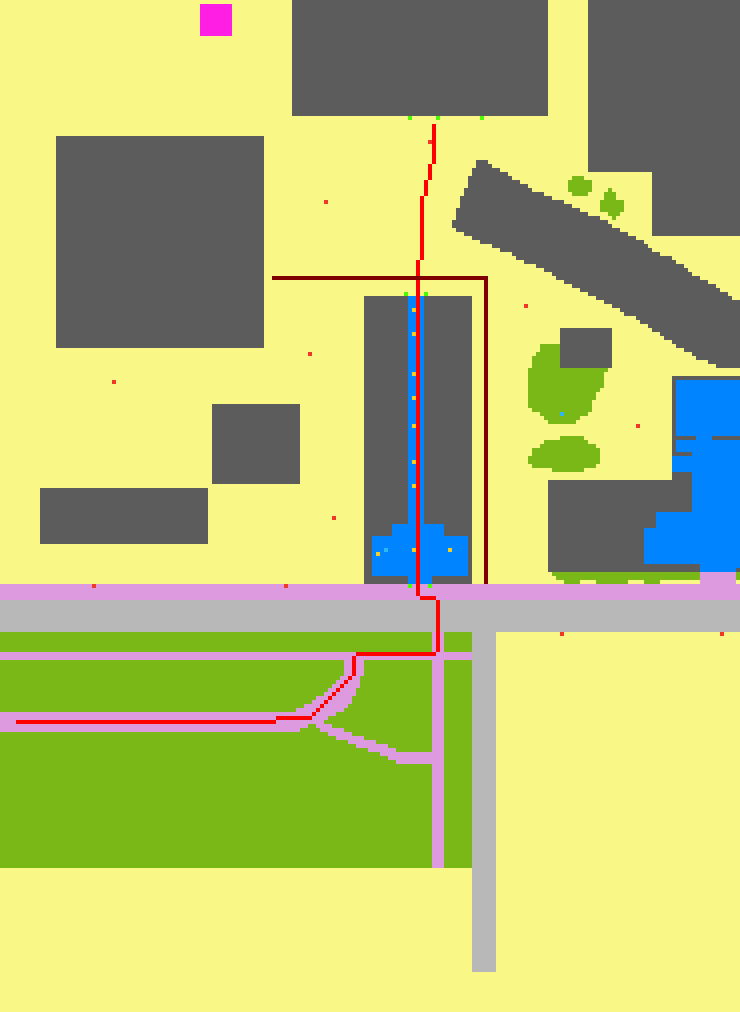
\includegraphics[width=\textwidth]{IST-Zustand}
        \caption{Modellierter IST-Zustand vom Campus}
        \label{img:IST}
	\end{figure}
	
\subsection{Maßnahmen zur Verbesserung des Campus}
Abbildung \ref{img:Verbesserung} zeigt den verbesserten Campus. Folgende Änderungen wurden dabei vorgenommen:

\begin{enumerate}
\item Gangbeleuchtung durch zusätzliche Lichtquellen verstärkt.
\item Leuchtstärke der Lichtquelle innerhalb des blauen Hauses erhöht.
\item Gang im blauen Haus verbreitert.
\item Mülleimer an den Eingängen zum blauen Haus versetzt (stehen nun nicht mehr direkt am Eingang).
\item Abwasserkanal am blauen Haus entfernt.
\item Zusätzliche Beleuchtung auf dem Weg von der U-Bahn zum blauen Haus eingefügt.
\item Zusätzliche Grünanlage auf dem Campus eingefügt.
\item Hinzufügen eines Access-Points im blauen Haus.
\end{enumerate}

	\begin{figure}[H]
                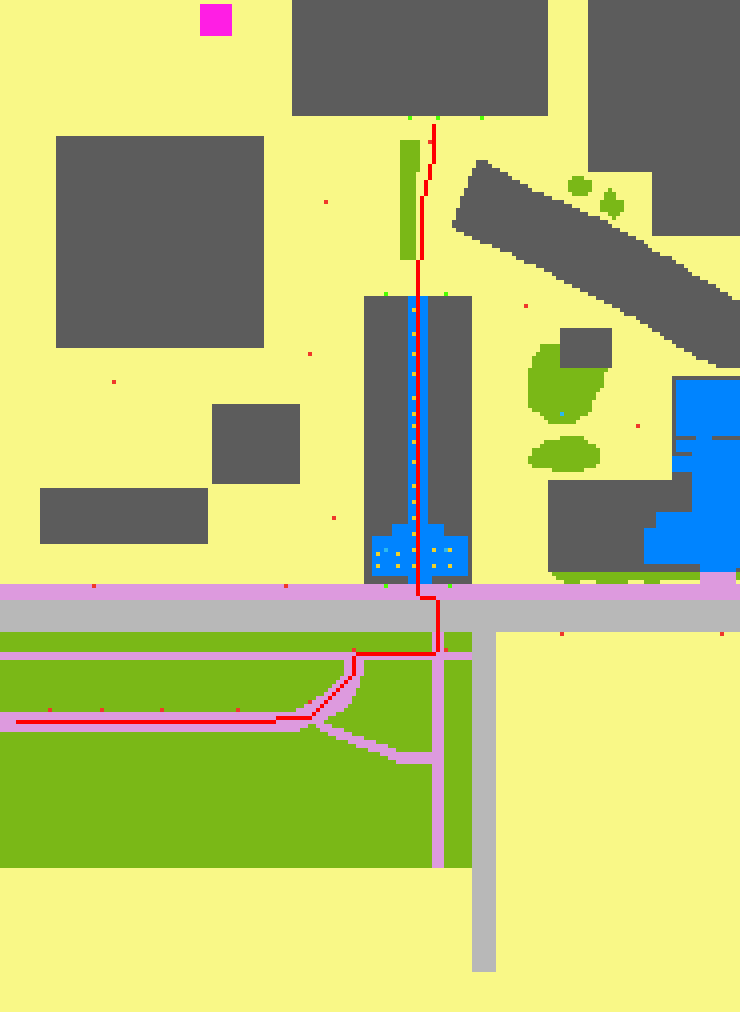
\includegraphics[width=\textwidth]{Verbesserung}
        \caption{Modellierter verbesserter Campus}
        \label{img:Verbesserung}
	\end{figure}
	
\subsection{Maßnahmen zur Verschlechterung des Campus}
Abbildung \ref{img:Verschlechterung} zeigt den verschlechterten Campus. Folgende Änderungen wurden dabei vorgenommen:

\begin{enumerate}
\item Müllcontainer zentral in dem Campus integriert.
\item Gang des blauen Hauses verkleinert.
\item Beleuchtung im Gang des blauen Hauses entfernt.
\item Straße vor dem blauen Haus verbreitert.
\item Weg von der U-Bahn zum blauen Haus verbreitert (hat zur Folge das weniger Grünanlage vorhanden ist).
\item Mülleimer im Gang des blauen Hauses und auf dem Weg zur U-Bahn hinzugefügt.
\item WLAN im blauen Haus entfernt.
\end{enumerate}

	\begin{figure}[H]
                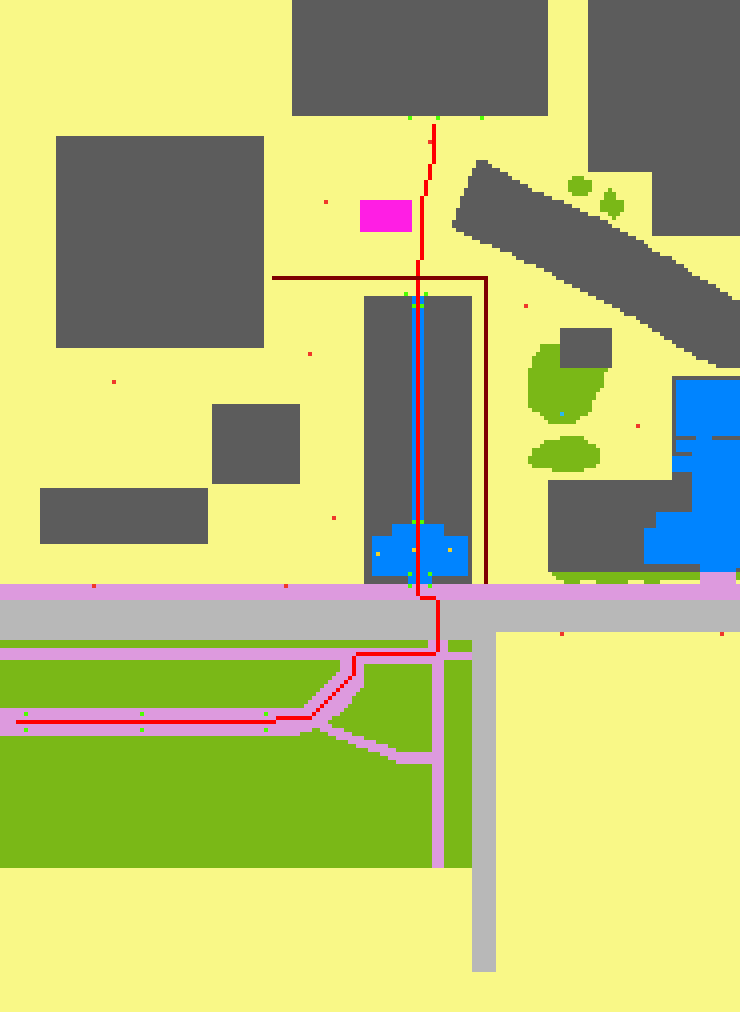
\includegraphics[width=\textwidth]{Verschlechterung}
        \caption{Modellierter verschlechterter Campus}
        \label{img:Verschlechterung}
	\end{figure}  

\section{Ergebnisse}\label{sec:Ergebnisse}
Abbildung \ref{img:Diagramme} zeigt die Visualisierung der durch die Simulation gewonnen Messergebnisse. Im folgenden Abschnitt wird auf die einzelnen Diagramme eingegangen und Auffälligkeiten erklärt.\\
Pro Diagramm werden die Kurven für Sicherheit, Produktivität, Soziologie und Vergnügen (Wohlfühlfaktor) gezeigt. Für eine vergrößerte Darstellung sei auf das angefügte \glqq Diagramme.pdf\grqq verwiesen.

	\begin{figure}[H]
                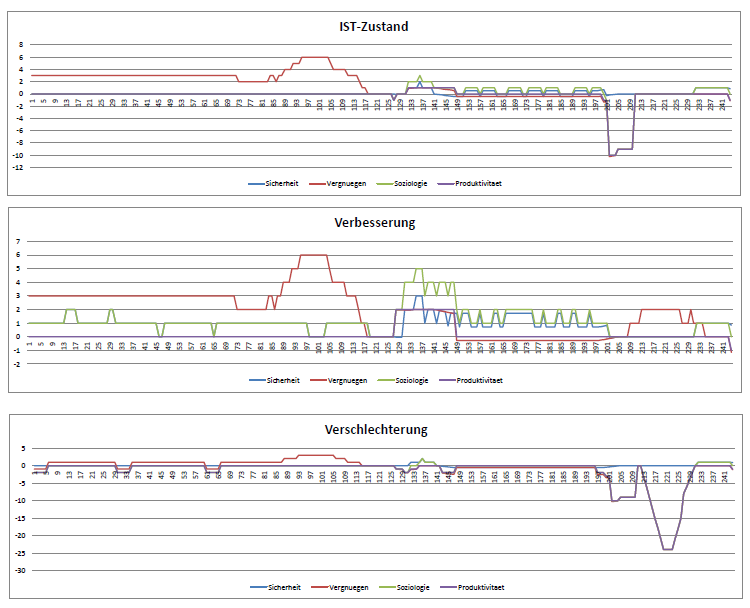
\includegraphics[width=\textwidth]{Diagramme/Diagramme.png}
        \caption{Simulationsergebnisse}
        \label{img:Diagramme}
	\end{figure} 

\subsection{IST-Zustand}
Beim Ist Zustand ist zu erkennen, dass das Vergnügen (rote Linie) auf dem Weg zur Uni im Vergleich zu den anderen Kennlinien stark erhöht ist. Dies ist durch den positiven Einfluss der Grünfläche auf dem Weg zur Uni zu erklären. Die Simulation wurde zu einer Uhrzeit durchgeführt zu der ein geringes Verkehrsaufkommen herrscht, wodurch der Einfluss der Straße auf das Sicherheitsempfinden des Agenten einen sehr geringen Einfluss hat. Bei den Schritten 133-137 gibt es ein Peak von Soziologie (grüne Linie) und Sicherheit (blaue Linie) welches sich mit dem vorhandenen Access-Point und den Lichtquellen im blauen Haus erklären lässt. Die Schritte 153-201 sind von kleinen Peaks im Soziologie und Sicherheitsempfinden geprägt. Dies liegt an den sporadisch verteilten Lichtquellen. Sicherheit und Vergnügen sind auf einem niedrigen Niveau konstant, was an der Enge des Ganges im blauen Haus liegt. Deutlich zu erkennen ist der Abfall in der Produktivität (lila Linie) welcher beim Überschreiten des Abwasserkanals stattfindet. Wir haben angenommen, dass sich starker Gestank negativ auf die Produktivität auswirkt. 

\subsection{Verbesserung}
In den Schritten 1-117 kann man eine Verbesserung auf der Sozioligieebene durch die zusätzlichen Lichtquellen auf dem Weg von der U-Bahn zur HAW erkennen. Die temporären Einbrüche lassen sich durch eine nicht gleichmäßige Verteilung der Beleuchtung erklären.
Die Verbesserungen der Produktivität in den Schritten 125-149 werden durch eine verbesserte WLAN Abdeckung hervorgerufen. Soziologie und Sicherheit steigen im gleichen Intervall, da die Ausleuchtung des Foyers verstärkt wurde. Gleiches gilt für die Schritte 149-201. Die stark fallende Produktivität im Bereich 201-210 war dem riechenden Abwasserkanal geschuldet. Dieser wurde entfernt; daher gibt es nun keinen Einbruch in der Produktivität mehr. Durch die Grünfläche oberhalb des blauen Gebäudes kann das Empfinden des Agenten auf der Vergnügungsebene in den Schritten 209-237 positiv beeinflusst werden.
   
\subsection{Verschlechterung}
In den Schritten 0-117 sinkt auf Grund der größeren Wegbreite der Einfluss der Grünflächen auf den Agenten, wodurch sein Empfinden auf der Vergnügungsebene geschmälert wird.
Durch die Mülleimer werden die negativen Ausschläge in der Vergnügen- und der Sicherheitsebene verursacht. Sie nehmen Platz weg und wirken sich so negativ auf die beiden Ebenen aus.\\
Die Entfernung der Beleuchtung im Gang führt dazu, dass sich Sicherheit und Vergnügen im Gegensatz zum IST-Zustand verringern. Die Einbrüche entstehen durch die neu hinzugekommen Mülleimer an den beiden Eingängen des Gebäude.
Die Schritte 197-210 beschreiben den Geruch der Mülleimer und des Kanals. Danach wird die Produktivität durch die verschobenen Müllcontainer negativ beeinflusst.

\section{Fazit}
Abschließend bleibt zu sagen, dass die Ergebnisse unsere Simulation sehr stark von den angenommen Parametern abhängen, die die getroffenen Veränderungen auf die Realität einschränken. Mülleimer wirken sich in unserem Modell in negativ auf das Vergnügen (wegen dem Geruch) des Agenten aus, können in der Realität aber durchaus auch einen positiven Effekt haben: saubere Wege. Dafür werden die Faktoren Licht und Platz besonders positiv vom Agenten aufgenommen, aber auch hier könnte zu viel Licht in der Realität einen negativen Effekt haben.

Um eine aussagekräftigere Simulation zu bekommen, müsste sowohl die Umwelt als auch der Agent weiter differenziert werden. Aufgrund der Tatsache, dass wir die Einflussfaktoren unserer Ebenen intuitiv gewählt und modelliert haben, ist ein recht einfaches Modell der Zielumgebung entstanden. Dadurch, dass genaue Kenntnisse über die Einflussfaktoren vorhanden sind, besteht die Gefahr durch gezielte Manipulation der Umgebung ein gewünschtes Ergebnis zu erlangen. In den verschiedenen Szenarien kann dies beispielhaft gezeigt werden, indem das Licht erhöht und damit ein positiver Einfluss auf die Sicherheit erzielt wird.


\end{document}

